\documentclass[tikz,border=7pt]{standalone}
\usepackage{tkz-euclide}
\usetkzobj{all} % on charge tous les objets

\begin{document}
  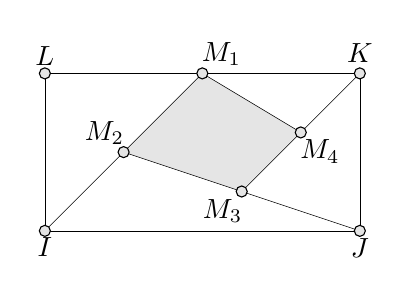
\begin{tikzpicture}[scale=2, every node/.style={circle, inner sep=1pt}]
    % définition des points
    \tkzDefPoints{0/0/I,2/0/J,2/1/K,0/1/L}
    \tkzDefMidPoint(K,L)\tkzGetPoint{M_1}
    \tkzDefMidPoint(I,M_1)\tkzGetPoint{M_2}
    \tkzDefMidPoint(J,M_2)\tkzGetPoint{M_3}
    \tkzDefMidPoint(K,M_3)\tkzGetPoint{M_4}
    % droites et segments
    \tkzDrawPolygon[fill, fill opacity=.1, draw=none](M_1,M_2,M_3,M_4)
    \tkzDrawPolygon(I,J,K,L)
    \tkzDrawSegments(I,M_1)
    \tkzDrawSegments(J,M_2)
    \tkzDrawSegments(K,M_3)
    \tkzDrawSegments(M_1,M_4)
    % marquage des points
    \tkzDrawPoints[size=4](I,J,K,L,M_1,M_2,M_3,M_4)
    \tkzLabelPoints[above](K,L)
    \tkzLabelPoints[above right](M_1)
    \tkzLabelPoints[above left](M_2)
    \tkzLabelPoints[below](I,J)
    \tkzLabelPoints[below left](M_3)
    \tkzLabelPoints[below right](M_4)
  \end{tikzpicture}
\end{document}
